%%   This file is part of the APS files in the REVTeX 4 distribution.
%%   Version 4.0 of REVTeX, August 2001
%%
%%
%%   Copyright (c) 2001 The American Physical Society.
%%
%%   See the REVTeX 4 README file for restrictions and more information.
%%
%
% This is a template for producing manuscripts for use with REVTEX 4.0
% Copy this file to another name and then work on that file.
% That way, you always have this original template file to use.
%
% Group addresses by affiliation; use superscriptaddress for long
% author lists, or if there are many overlapping affiliations.
% For Phys. Rev. appearance, change preprint to twocolumn.
% Choose pra, prb, prc, prd, pre, prl, prstab, or rmp for journal
%  Add 'draft' option to mark overfull boxes with black boxes
%  Add 'showpacs' option to make PACS codes appear

% Edited by Camilla Harris Jan 2015
% For use by Camilla Harris, Akshat Mahajan
% in creating Lab Reports for 180c at UCLA
% this file and auxiliary files were retrieved from
% http://www-d0.fnal.gov/Run2Physics/WWW/templates/
% on Jan 19 2015

\documentclass[aps,prl,twocolumn,superscriptaddress,groupedaddress]{revtex4}  % for review and submission
%\documentclass[aps,preprint,superscriptaddress,groupedaddress]{revtex4}  % for double-spaced preprint
% CAMILLA: I removed the PACS functionality
\usepackage{graphicx}  % needed for figures
	%if using postscript files compile with XeLaTex
\usepackage{dcolumn}   % needed for some tables
\usepackage{bm}        % for math
\usepackage{amssymb}   % for math

% avoids incorrect hyphenation, added Nov/08 by SSR
\hyphenation{ALPGEN}
\hyphenation{EVTGEN}
\hyphenation{PYTHIA}


\begin{document}
\title{Template for 180c Reports}
\input author_list.tex        % includes institutions and visitors
\date{\today}


\begin{abstract}
An article usually includes an abstract, a concise summary of the work
covered at length in the main body of the article. It is used for
secondary publications and for information retrieval purposes.
For PRL, the rule of thumb is that the abstract should be less than
8 lines and the text (excluding authors, abstract but including tables,
figures and references) should be less than 4 pages (leave about 20 lines
empty on page 4) in two-column format.
PRL and PRD papers have to have PACS (Phsyics and Astronomy Classification
Scheme) numbers. Please see {\tt http://www.aip.org/pacs/} for the numbers
relevant to your paper. A set of standard references can be found at the
end of this example paper. \textbf{Use this document as default template.}
\end{abstract}

\maketitle

\section{\label{sec:level1}First-level heading}

This sample document demonstrates proper use of REV\TeX~4 (and
\LaTeXe) in mansucripts prepared for submission to APS
journals. Further information can be found in the REV\TeX~4
documentation included in the distribution or available at
\url{http://publish.aps.org/revtex4/}.

When commands are referred to in this example file, they are always
shown with their required arguments, using normal \TeX{} format. In
this format, \verb+#1+, \verb+#2+, etc. stand for required
author-supplied arguments to commands. For example, in
\verb+\section{#1}+ the \verb+#1+ stands for the title text of the
author's section heading, and in \verb+\title{#1}+ the \verb+#1+
stands for the title text of the paper.

Line breaks in section headings at all levels can be introduced using
\textbackslash\textbackslash. A blank input line tells \TeX\ that the
paragraph has ended. Note that top-level section headings are
automatically uppercased. If a specific letter or word should appear in
lowercase instead, you must escape it using \verb+\lowercase{#1}+ as
in the word ``via'' above.

\subsection{\label{sec:level2}Second-level heading: Formatting}

This file may be formatted in both the \texttt{preprint} and
\texttt{twocolumn} styles. \texttt{twocolumn} format may be used to
mimic final journal output. Either format may be used for submission
purposes; however, for peer review and production, APS will format the
article using the \texttt{preprint} class option. Hence, it is
essential that authors check that their manuscripts format acceptably
under \texttt{preprint}. Manuscripts submitted to APS that do not
format correctly under the \texttt{preprint} option may be delayed in
both the editorial and production processes.

The \texttt{widetext} environment will make the text the width of the
full page.  The width-changing commands only take effect in \texttt{twocolumn}
formatting. It has no effect if \texttt{preprint} formatting is chosen
instead.

To cite bibliography entries, use the \verb+\cite{#1}+ command. Most
journal styles will display the corresponding number(s) in square
brackets: \cite{d0det}. To avoid the square brackets, use
\verb+\onlinecite{#1}+: Refs.~\onlinecite{d0det} and
\onlinecite{geant,pythia}. REV\TeX\ ``collapses'' lists of
consecutive reference numbers where possible. We now cite everyone
together \cite{geant, pythia, cteq}, and once again
(Refs.~\onlinecite{geant, pythia, cteq}). Note that the references
were also sorted into the correct numerical order as well.

Footnotes are produced using the \verb+\footnote{#1}+ command. Most
APS journal styles put footnotes into the bibliography. REV\TeX~4 does
this as well, but instead of interleaving the footnotes with the
references, they are listed at the end of the references. Because the correct
numbering of the footnotes must occur after the numbering of the
references, an extra pass of \LaTeX\ is required in order to get the
numbering correct.


Inline math may be typeset using the \verb+$+ delimiters. Bold math
symbols may be achieved using the \verb+bm+ package and the
\verb+\bm{#1}+ command it supplies. For instance, a bold $\alpha$ can
be typeset as \verb+$\bm{\alpha}$+ giving $\bm{\alpha}$. Fraktur and
Blackboard (or open face or double struck) characters should be
typeset using the \verb+\mathfrak{#1}+ and \verb+\mathbb{#1}+ commands
respectively. Both are supplied by the \texttt{amssymb} package. For
example, \verb+$\mathbb{R}$+ gives $\mathbb{R}$ and
\verb+$\mathfrak{G}$+ gives $\mathfrak{G}$

In \LaTeX\ there are many different ways to display equations, and a
few preferred ways are noted below. Displayed math will center by
default. Use the class option \verb+fleqn+ to flush equations left.

Below we have numbered single-line equations; this is the most common
type of equation in \textit{Physical Review}:
\begin{eqnarray}
\chi_+(p)\alt{\bf [}2|{\bf p}|(|{\bf p}|+p_z){\bf ]}^{-1/2}
\left(
\begin{array}{c}
|{\bf p}|+p_z\\
px+ip_y
\end{array}\right)\;,
\\
\left\{%
 \openone234567890abc123\alpha\beta\gamma\delta1234556\alpha\beta
 \frac{1\sum^{a}_{b}}{A^2}%
\right\}%
\label{eq:one}.
\end{eqnarray}
Note the open one in Eq.~(\ref{eq:one}).

Not all numbered equations will fit within a narrow column this
way. The equation number will move down automatically if it cannot fit
on the same line with a one-line equation:
\begin{equation}
\left\{
 ab12345678abc123456abcdef\alpha\beta\gamma\delta1234556\alpha\beta
 \frac{1\sum^{a}_{b}}{A^2}%
\right\}.
\end{equation}

When the \verb+\label{#1}+ command is used [cf. input for
Eq.~(\ref{eq:one})], the equation can be referred to in text without
knowing the equation number that \TeX\ will assign to it. Just
use \verb+\ref{#1}+, where \verb+#1+ is the same name that used in
the \verb+\label{#1}+ command.

Unnumbered single-line equations can be typeset
using the \verb+\[+, \verb+\]+ format:
\[g^+g^+ \rightarrow g^+g^+g^+g^+ \dots ~,~~q^+q^+\rightarrow
q^+g^+g^+ \dots ~. \]


Figures may be inserted by using either the \texttt{graphics} or
\texttt{graphicx} packages. These packages both define the
\verb+\includegraphics{#1}+ command, but they differ in how optional
arguments for specifying the orientation, scaling, and translation of the
figure. Fig.~\ref{fig:epsart} shows a figure that is small enough to
fit in a single column. It is embedded using the \texttt{figure}
environment which provides both the caption and the imports the figure
file.

\begin{figure}

\includegraphics[scale=0.8]{fig_1.png}
\caption{\label{fig:epsart} A figure caption. The figure captions are
automatically numbered.}
\end{figure}

Fig.~\ref{fig:wide} is a figure that is too wide for a single column,
so instead the \texttt{figure*} environment has been used.
\begin{figure*}
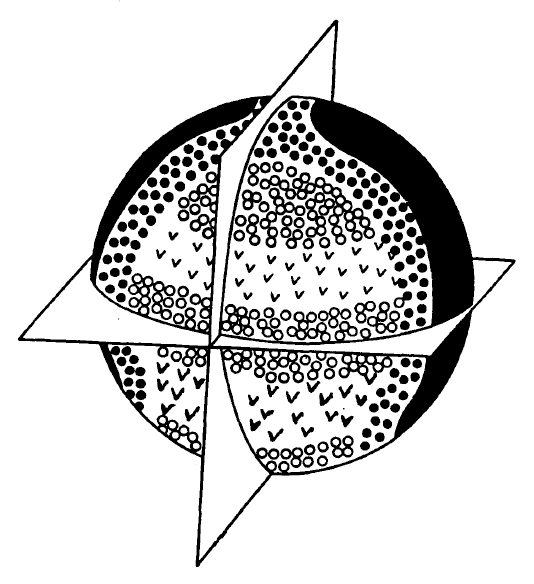
\includegraphics{fig_2.png}
\caption{\label{fig:wide}Use the figure* environment to get a wide
figure that spans the page in \texttt{twocolumn} formatting.}
\end{figure*}


The heart of any table is the \texttt{tabular} environment which gives
the rows of the tables. Each row consists of column entries separated
by \verb+&+'s and terminates with \textbackslash\textbackslash. The
required argument for the \texttt{tabular} environment
specifies how data are displayed in the columns. For instance, entries
may be centered, left-justified, right-justified, aligned on a decimal
point. Extra column-spacing may be be specified as well, although
REV\TeX~4 sets this spacing so that the columns fill the width of the
table. Horizontal rules are typeset using the \verb+\hline+
command. The doubled (or Scotch) rules that appear at the top and
bottom of a table can be achieved enclosing the \texttt{tabular}
environment within a \texttt{ruledtabular} environment. Rows whose
columns span multiple columns can be typeset using the
\verb+\multicolumn{#1}{#2}{#3}+ command (for example, see the first
row of Table~\ref{tab:table3}).

Tables~\ref{tab:table1}-\ref{tab:table4} show various effects. Tables
that fit in a narrow column are contained in a \texttt{table}
environment. Table~\ref{tab:table3} is a wide table set with the
\texttt{table*} environment. Long tables may need to break across
pages. The most straightforward way to accomplish this is to specify
the \verb+[H]+ float placement on the \texttt{table} or
\texttt{table*} environment. However, the standard \LaTeXe\ package
\texttt{longtable} will give more control over how tables break and
will allow headers and footers to be specified for each page of the
table. A simple example of the use of \texttt{longtable} can be found
in the file \texttt{summary.tex} that is included with the REV\TeX~4
distribution.

There are two methods for setting footnotes within a table (these
footnotes will be displayed directly below the table rather than at
the bottom of the page or in the bibliography). The easiest
and preferred method is just to use the \verb+\footnote{#1}+
command. This will automatically enumerate the footnotes with
lowercase roman letters. However, it is sometimes necessary to have
multiple entries in the table share the same footnote. In this case,
there is no choice but to manually create the footnotes using
\verb+\footnotemark[#1]+ and \verb+\footnotetext[#1]{#2}+.
\texttt{\#1} is a numeric value. Each time the same value for
\texttt{\#1} is used, the same mark is produced in the table. The
\verb+\footnotetext[#1]{#2}+ commands are placed after the \texttt{tabular}
environment. Examine the \LaTeX\ source and output for
Tables~\ref{tab:table1} and \ref{tab:table2} for examples.

\begin{table}
\caption{\label{tab:table1}This is a narrow table which fits into a
narrow column when using \texttt{twocolumn} formatting. Note that
REV\TeX~4 adjusts the intercolumn spacing so that the table fills the
entire width of the column. Table captions are numbered
automatically. This table illustrates left-aligned, centered, and
right-aligned columns.  }
\begin{ruledtabular}
\begin{tabular}{lcr}
Left\footnote{Note a.}&Centered\footnote{Note b.}&Right\\
\hline
1 & 2 & 3\\
10 & 20 & 30\\
100 & 200 & 300\\
\end{tabular}
\end{ruledtabular}
\end{table}

\begin{table}
\caption{\label{tab:table2}A table with more columns still fits
properly in a column. Note that several entries share the same
footnote. Inspect the \LaTeX\ input for this table to see
exactly how it is done.}
\begin{ruledtabular}
\begin{tabular}{cccccccc}
 &$r_c$ (\AA)&$r_0$ (\AA)&$\kappa r_0$&
 &$r_c$ (\AA) &$r_0$ (\AA)&$\kappa r_0$\\
\hline
Cu& 0.800 & 14.10 & 2.550 &Sn\footnotemark[1]
& 0.680 & 1.870 & 3.700 \\
Ag& 0.990 & 15.90 & 2.710 &Pb\footnotemark[2]
& 0.450 & 1.930 & 3.760 \\
Au& 1.150 & 15.90 & 2.710 &Ca\footnotemark[3]
& 0.750 & 2.170 & 3.560 \\
Mg& 0.490 & 17.60 & 3.200 &Sr\footnotemark[4]
& 0.900 & 2.370 & 3.720 \\
Zn& 0.300 & 15.20 & 2.970 &Li\footnotemark[2]
& 0.380 & 1.730 & 2.830 \\
Cd& 0.530 & 17.10 & 3.160 &Na\footnotemark[5]
& 0.760 & 2.110 & 3.120 \\
Hg& 0.550 & 17.80 & 3.220 &K\footnotemark[5]
&  1.120 & 2.620 & 3.480 \\
Al& 0.230 & 15.80 & 3.240 &Rb\footnotemark[3]
& 1.330 & 2.800 & 3.590 \\
Ga& 0.310 & 16.70 & 3.330 &Cs\footnotemark[4]
& 1.420 & 3.030 & 3.740 \\
In& 0.460 & 18.40 & 3.500 &Ba\footnotemark[5]
& 0.960 & 2.460 & 3.780 \\
Tl& 0.480 & 18.90 & 3.550 & & & & \\
\end{tabular}
\end{ruledtabular}
\footnotetext[1]{Here's the first, from Ref.~\onlinecite{pdg}.}
\footnotetext[2]{Here's the second.}
\footnotetext[3]{Here's the third.}
\footnotetext[4]{Here's the fourth.}
\footnotetext[5]{And etc.}
\end{table}

\begin{table*}
\caption{\label{tab:table3}This is a wide table that spans the page
width in \texttt{twocolumn} mode. It is formatted using the
\texttt{table*} environment. It also demonstates the use of
\textbackslash\texttt{multicolumn} in rows with entries that span
more than one column.}
\begin{ruledtabular}
\begin{tabular}{ccccc}
 &\multicolumn{2}{c}{$D_{4h}^1$}&\multicolumn{2}{c}{$D_{4h}^5$}\\
 Ion&1st alternative&2nd alternative&lst alternative
&2nd alternative\\ \hline
 K&$(2e)+(2f)$&$(4i)$ &$(2c)+(2d)$&$(4f)$ \\
 Mn&$(2g)$\footnote{The $z$ parameter of these positions is $z\sim\frac{1}{4}$.}
 &$(a)+(b)+(c)+(d)$&$(4e)$&$(2a)+(2b)$\\
 Cl&$(a)+(b)+(c)+(d)$&$(2g)$\footnotemark[1]
 &$(4e)^{\text{a}}$\\
 He&$(8r)^{\text{a}}$&$(4j)^{\text{a}}$&$(4g)^{\text{a}}$\\
 Ag& &$(4k)^{\text{a}}$& &$(4h)^{\text{a}}$\\
\end{tabular}
\end{ruledtabular}
\end{table*}

\begin{table}
\caption{\label{tab:table4}Numbers in columns Three--Five have been
aligned by using the ``d'' column specifier (requires the
\texttt{dcolumn} package). Non-numeric entries (those entries without
a ``.'') in a ``d'' column are aligned on the decimal point. Use the
``D'' specifier for more complex layouts. }
\begin{ruledtabular}
\begin{tabular}{ccddd}
One&Two&\mbox{Three}&\mbox{Four}&\mbox{Five}\\
\hline
one&two&\mbox{three}&\mbox{four}&\mbox{five}\\
He&2& 2.77234 & 45672. & 0.69 \\
C\footnote{Some tables require footnotes.}
  &C\footnote{Some tables need more than one footnote.}
  & 12537.64 & 37.66345 & 86.37 \\
\end{tabular}
\end{ruledtabular}
\end{table}



\textit{Physical Review} style requires that the initial citation of
figures or tables be in numerical order in text, so don't cite
Fig.~\ref{fig:wide} until Fig.~\ref{fig:epsart} has been cited.



%\input acknowledgement.tex   % input acknowledgement
								   % a simple paragraph, no formatting

\begin{thebibliography}{99}

  \bibitem{d0det}
    Standard D\O\ detector reference:  \\
V.M.~Abazov {\sl et al.} (D0 Collaboration),
Nucl. Instrum. Methods Phys. Res. A {\bf 565}, 463  (2006).

  \bibitem{d0lumi}
    ** New ** D\O\ luminosity reference: \\
T.~Andeen {\sl et al.}, FERMILAB-TM-2365 (2007).

  \bibitem{pdg}
   Particle Data Group reference: \\
   W.-M.~Yao {\sl et al.}, Journal of Physics G {\bf 33}, 1 (2006).

  \bibitem{geant}
    {\sc Geant} reference: \\
    R. Brun and F. Carminati, CERN Program Library Long Writeup W5013, 1993 (unpublished).

  \bibitem{pythia}
    {\sc Pythia} reference: \\
    T. Sj\"{o}strand {\sl et al.}, Comput. Phys. Commun. {\bf 135}, 238 (2001).

  \bibitem{cteq}
    {\sc Cteq6} reference: \\
    J. Pumplin {\sl et al.}, JHEP {\bf 0207} 012 (2002) and
    D. Stump {\sl et al.}, JHEP {\bf 0310} 046 (2003).

  \bibitem{cls}
    LEP CL$_S$ reference: \\
    T. Junk, Nucl. Instrum. Methods A {\bf 434}, 435 (1999).

  \bibitem{d0limit}
   D\O\ Bayesian reference: \\
   I. Bertram {\sl et al.}, FERMILAB-TM-2104 (2000).

  \bibitem{d0jets}
  D\O\ cone-jet reference: \\
G.C.~Blazey {\it et al.}, in
{\sl Proceedings of the Workshop: QCD and Weak Boson
Physics in Run II,} edited by U.~Baur, R.K.~Ellis, and
D. Zeppenfeld, Fermilab-Pub-00/297 (2000).

\end{thebibliography}

\end{document}
